% Created 2021-08-18 Wed 12:42
% Intended LaTeX compiler: pdflatex
\documentclass[11pt]{article}
\usepackage[utf8]{inputenc}
\usepackage[T1]{fontenc}
\usepackage{graphicx}
\usepackage{grffile}
\usepackage{longtable}
\usepackage{wrapfig}
\usepackage{rotating}
\usepackage[normalem]{ulem}
\usepackage{amsmath}
\usepackage{textcomp}
\usepackage{amssymb}
\usepackage{capt-of}
\usepackage{hyperref}
\author{David Lewis}
\date{\today}
\title{}
\hypersetup{
 pdfauthor={David Lewis},
 pdftitle={},
 pdfkeywords={},
 pdfsubject={},
 pdfcreator={Emacs 28.0.50 (Org mode 9.5)}, 
 pdflang={English}}
\begin{document}

\tableofcontents

\section{Abstract}
\label{sec:org2436a26}
\section{Introduction}
\label{sec:orgdb000b1}
\section{Methods}
\label{sec:org3555088}
\subsection{Transcriptomic Workflow Overview}
\label{sec:orgf99f715}
\begin{center}
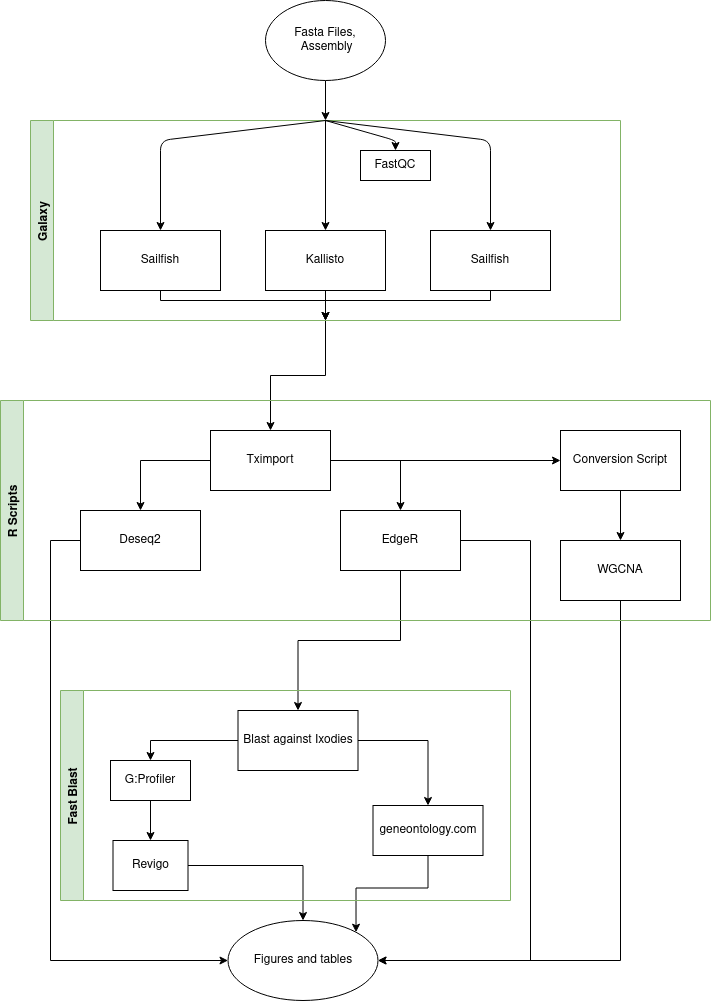
\includegraphics[width=.9\linewidth]{Workflow.png}
\end{center}
\subsubsection{Quantification}
\label{sec:org83bca1e}
The Raw high-throughput RNA-sequencing data from each trial were saved as individual FASTQ files.
The FASTQ files were uploaded to the Galaxy platform (\texttt{usegalaxy.org} ) where the quantifiaction occured.
First, Galaxy's 'FastQC' tool was used to determine the quality of the raw data and to mitigate the effects of amplification bias \texttt{insert settings here}). The Kmer test within 'FastQC' was enabled and set at a length of 7bp.
Following this initial quality-check, the raw files were trimmed with 'Trimmomatic' using its default settings (\texttt{description}).
FastQC was run on the trimmed files to confirm its quality.

After the data was trimmed, transcript abundance quantifiaction was performed by the Galaxy's 'Sailfish quant' tool using the default settings (\texttt{description}).
\subsection{Differential expression analysis}
\label{sec:org8f25798}
DESeq2(\texttt{Reference}) and EdgeR(\texttt{Reference}) were used to test for differential expression between the legs, body, and pesticide treatment (Deet and Perm).
The differential analysis becomes more reliable when the results of the similar tools are compared.


\subsection{WGCNA}
\label{sec:orgc01e2c7}
\subsection{GO analysis}
\label{sec:org57e0974}
\subsubsection{Blast}
\label{sec:org23bbd76}

\subsubsection{GProfiler}
\label{sec:org0591d33}
functional enrichment analysis. The output from Blast is sent to GProfiler. The GProfiler output is sent to revigo.
\subsubsection{Revigo}
\label{sec:orgf961e1d}
The R script output of Revigo generates tree-maps of the genes.
\subsubsection{Geneontolyg.org}
\label{sec:org1318598}
The ouptut of blast is sent to Geneontology.org
\section{Results}
\label{sec:orged1e4f7}
\subsection{Figure 1: methods comparison between EdgeR and Deseq2}
\label{sec:org94490e8}
This figure compares the expression data that is present in both EdgeR and Deseq2. The P value is small, indicating that EdgeR and Deseq2 have similar results.
\begin{center}
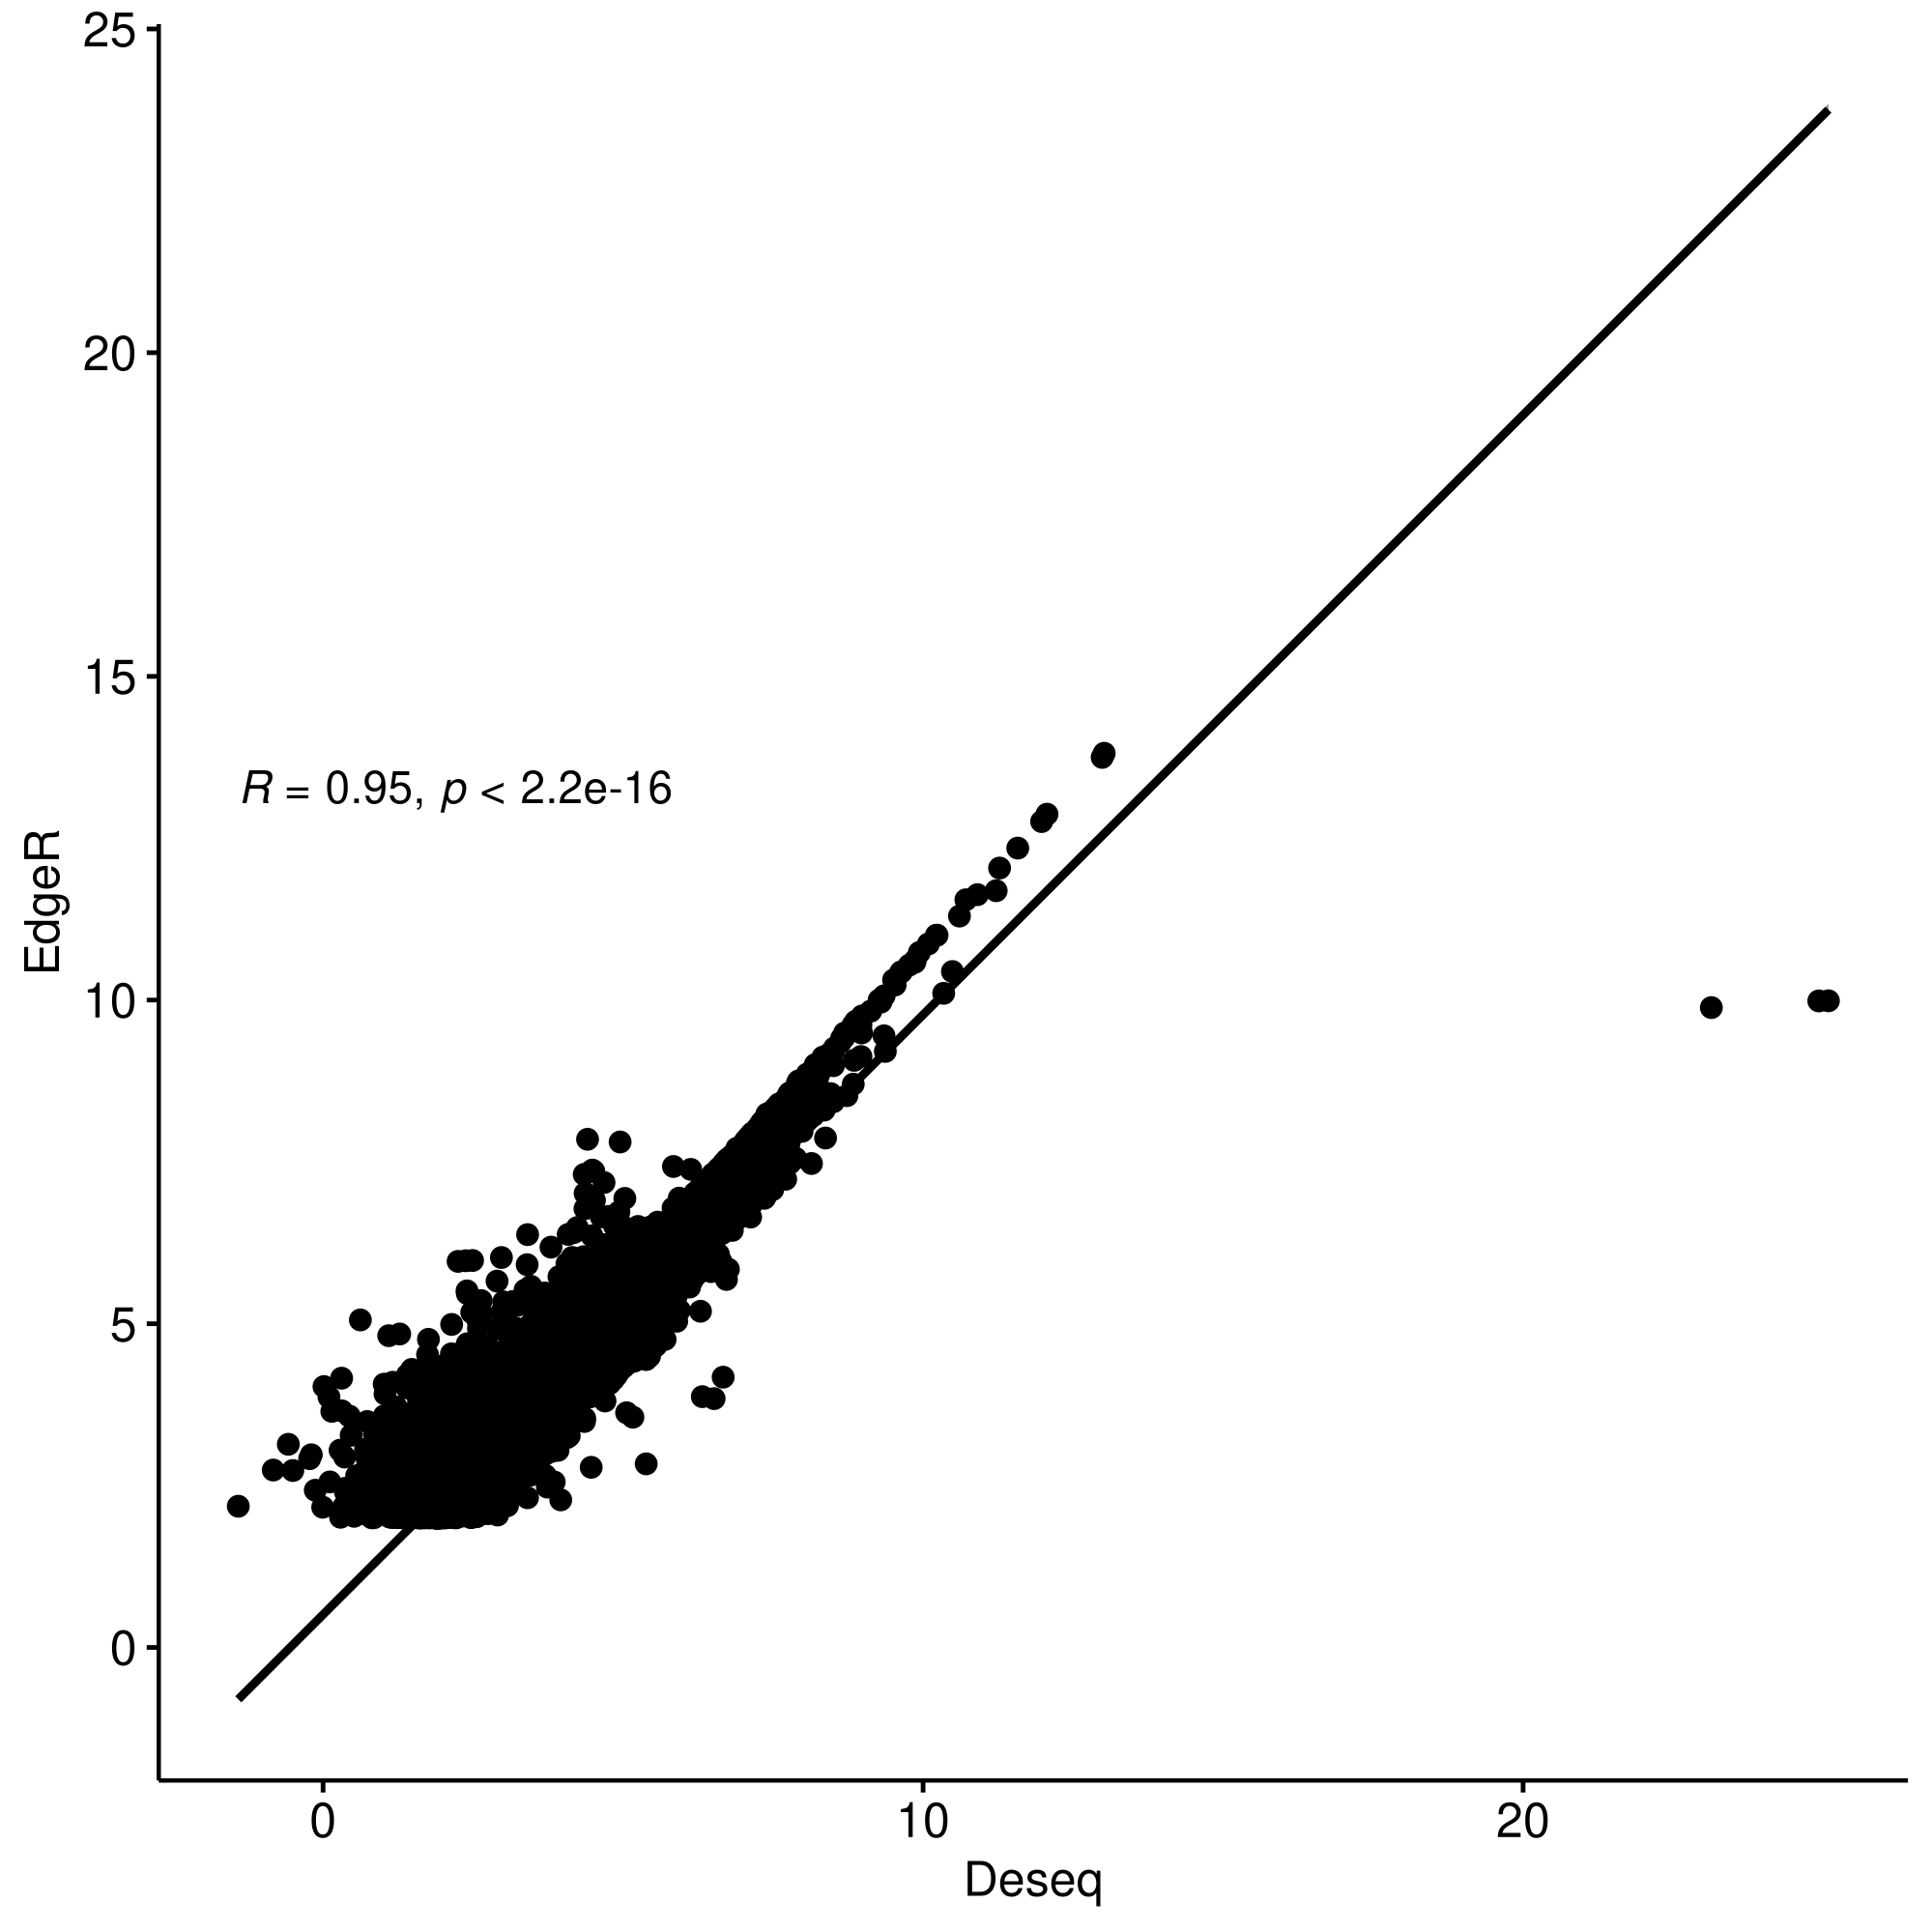
\includegraphics[width=0.6\textwidth]{figure1/pearson.png}
\captionof{figure}{The quantification files were run through both EdgeR and Deseq2. Each axis plots the expression values as given by its respective title.}
\end{center}
\subsection{Figure 2: Perm and Deet repellency and survival}
\label{sec:org5e9c6e4}
\subsection{Figure 3: Leg vs Body general (control)}
\label{sec:orgcc87d3d}
This figure compares the genes up-regulated in the body and leg compared to the total number of genes from the sample.
\begin{center}
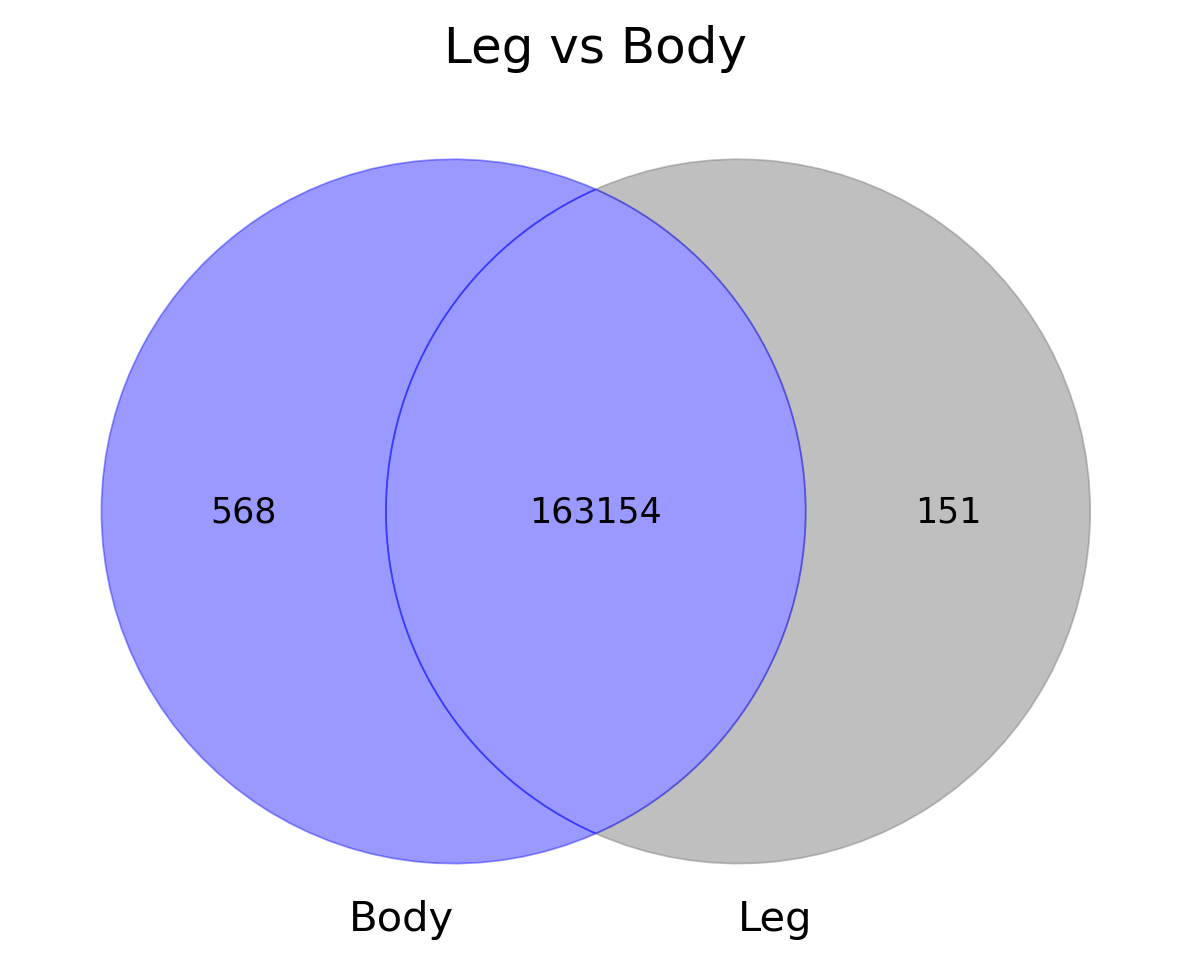
\includegraphics[width=.9\linewidth]{figure3/Deseq-BodyvsLeg.png}
\end{center}
\subsubsection{{\bfseries\sffamily TODO} supplemental tables}
\label{sec:orgd4fd707}
\subsection{Figure 4: Leg vs Body Specifics overlap with Ixodies}
\label{sec:org8ef8d3e}
Refer to paper in google drive. Discussion.
\subsection{Figure 5:Response to DEET In Leg and Body}
\label{sec:orgbe7f4d3}
\subsubsection{Body}
\label{sec:orgdfd6335}
\begin{center}
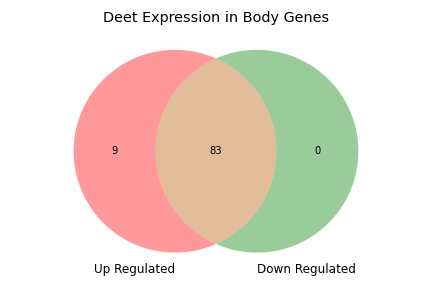
\includegraphics[width=.9\linewidth]{figure5/DeetBodyDeseq.png}
\end{center}
\subsubsection{Leg}
\label{sec:org5cb2400}
\begin{center}
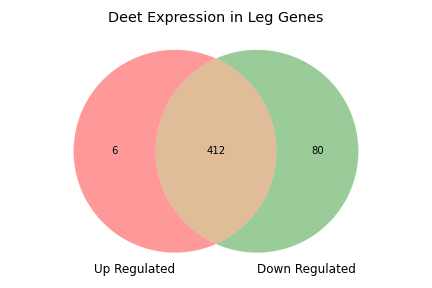
\includegraphics[width=.9\linewidth]{figure5/DeetLegDeseq.png}
\end{center}
\subsubsection{{\bfseries\sffamily TODO} supplemental tables}
\label{sec:orgcd02d67}
\subsection{Figure 6: Response to PERM in Leg and Body}
\label{sec:orga8451c9}
\subsubsection{Body}
\label{sec:orgdae8c46}
\begin{center}
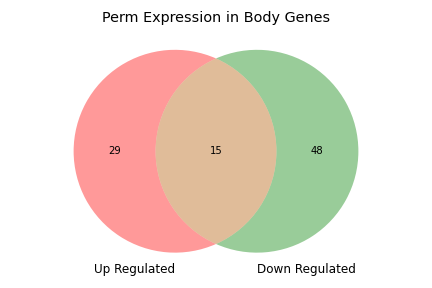
\includegraphics[width=.9\linewidth]{figure6/PermBodyDeseq.png}
\end{center}
\subsubsection{Leg}
\label{sec:orgd72c1e6}
\begin{center}
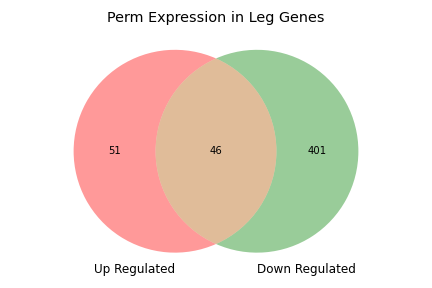
\includegraphics[width=.9\linewidth]{figure6/PermLegDeseq.png}
\end{center}
\subsubsection{{\bfseries\sffamily TODO} supplemental tables}
\label{sec:orgc60d674}
\subsection{Figure 7: WGCNA}
\label{sec:org72176c5}
\subsection{Figure 8: Overlap Between the response, body and leg}
\label{sec:org16011ef}
Don't think we need it now.
\subsection{Figure 9: Time Course Legs}
\label{sec:orgef7159c}
\subsubsection{DEET}
\label{sec:org5eb2e98}
\begin{center}
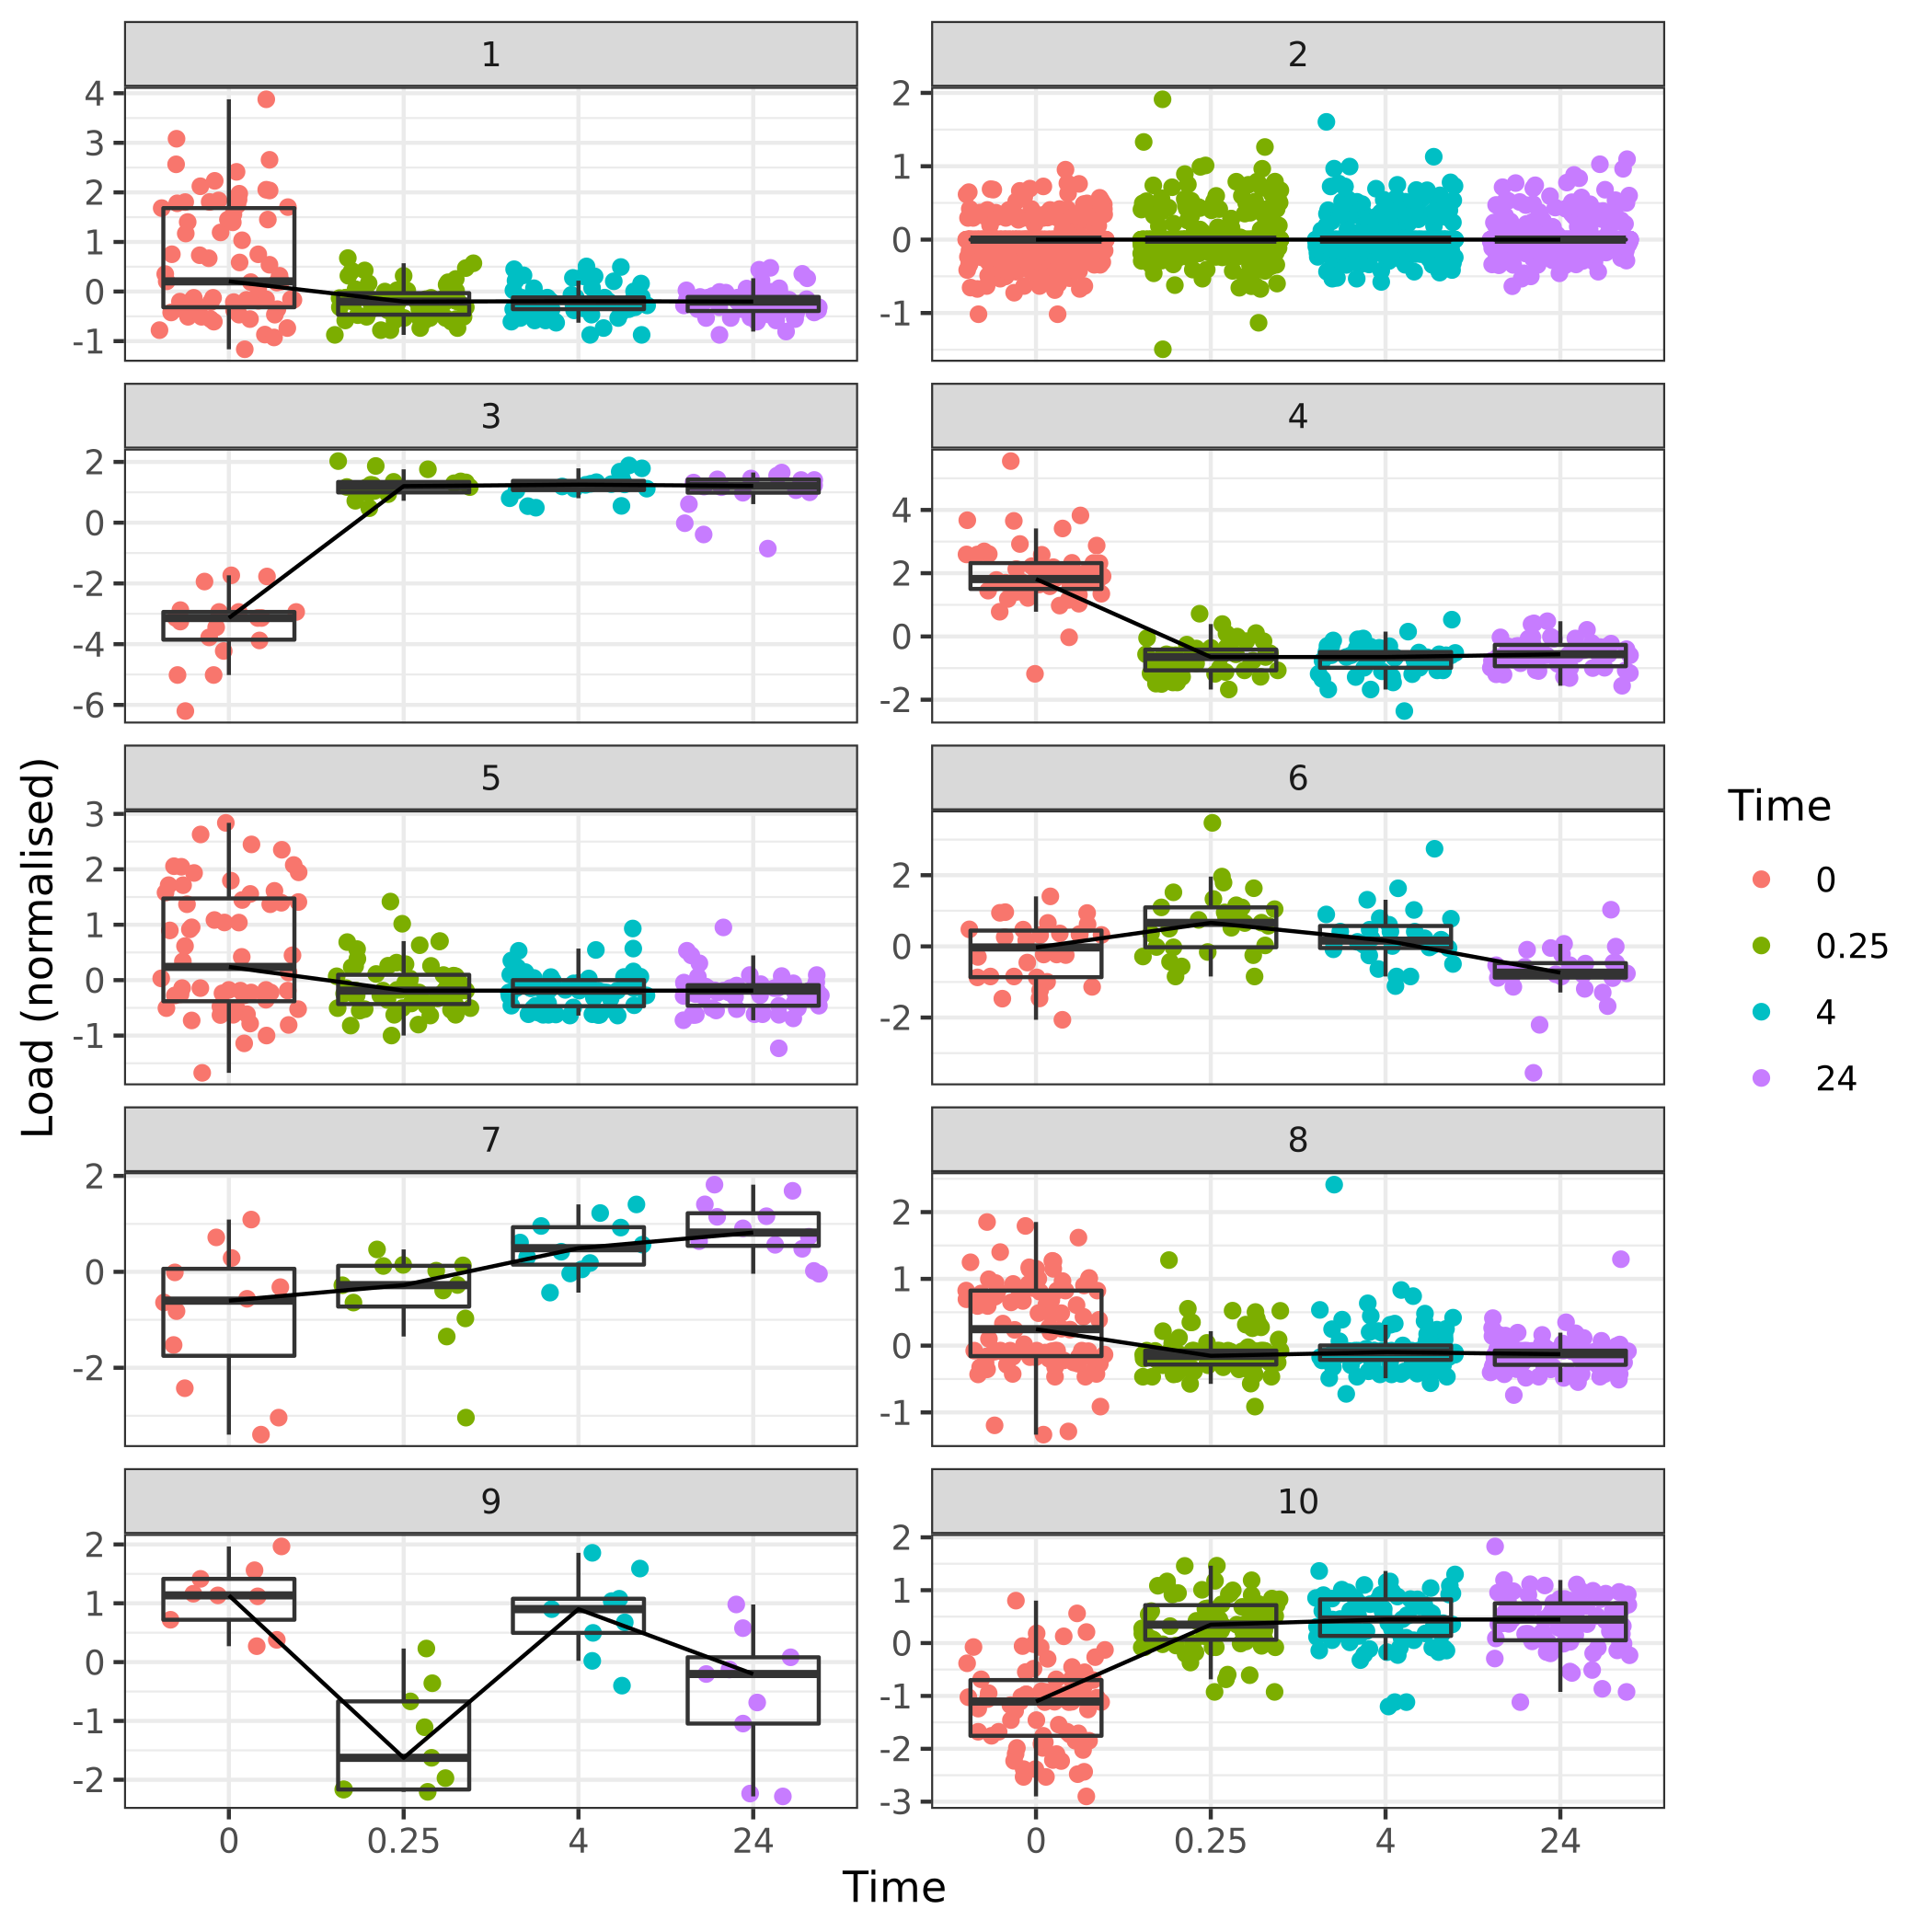
\includegraphics[width=.9\linewidth]{figure9/DEET/Legbox.png}
\end{center}
\begin{enumerate}
\item Supplemental Tables
\label{sec:orgc722011}
\url{figure9/DEET/Legbox}
\end{enumerate}
\subsubsection{PERM}
\label{sec:orgb3a3f0b}
\begin{center}
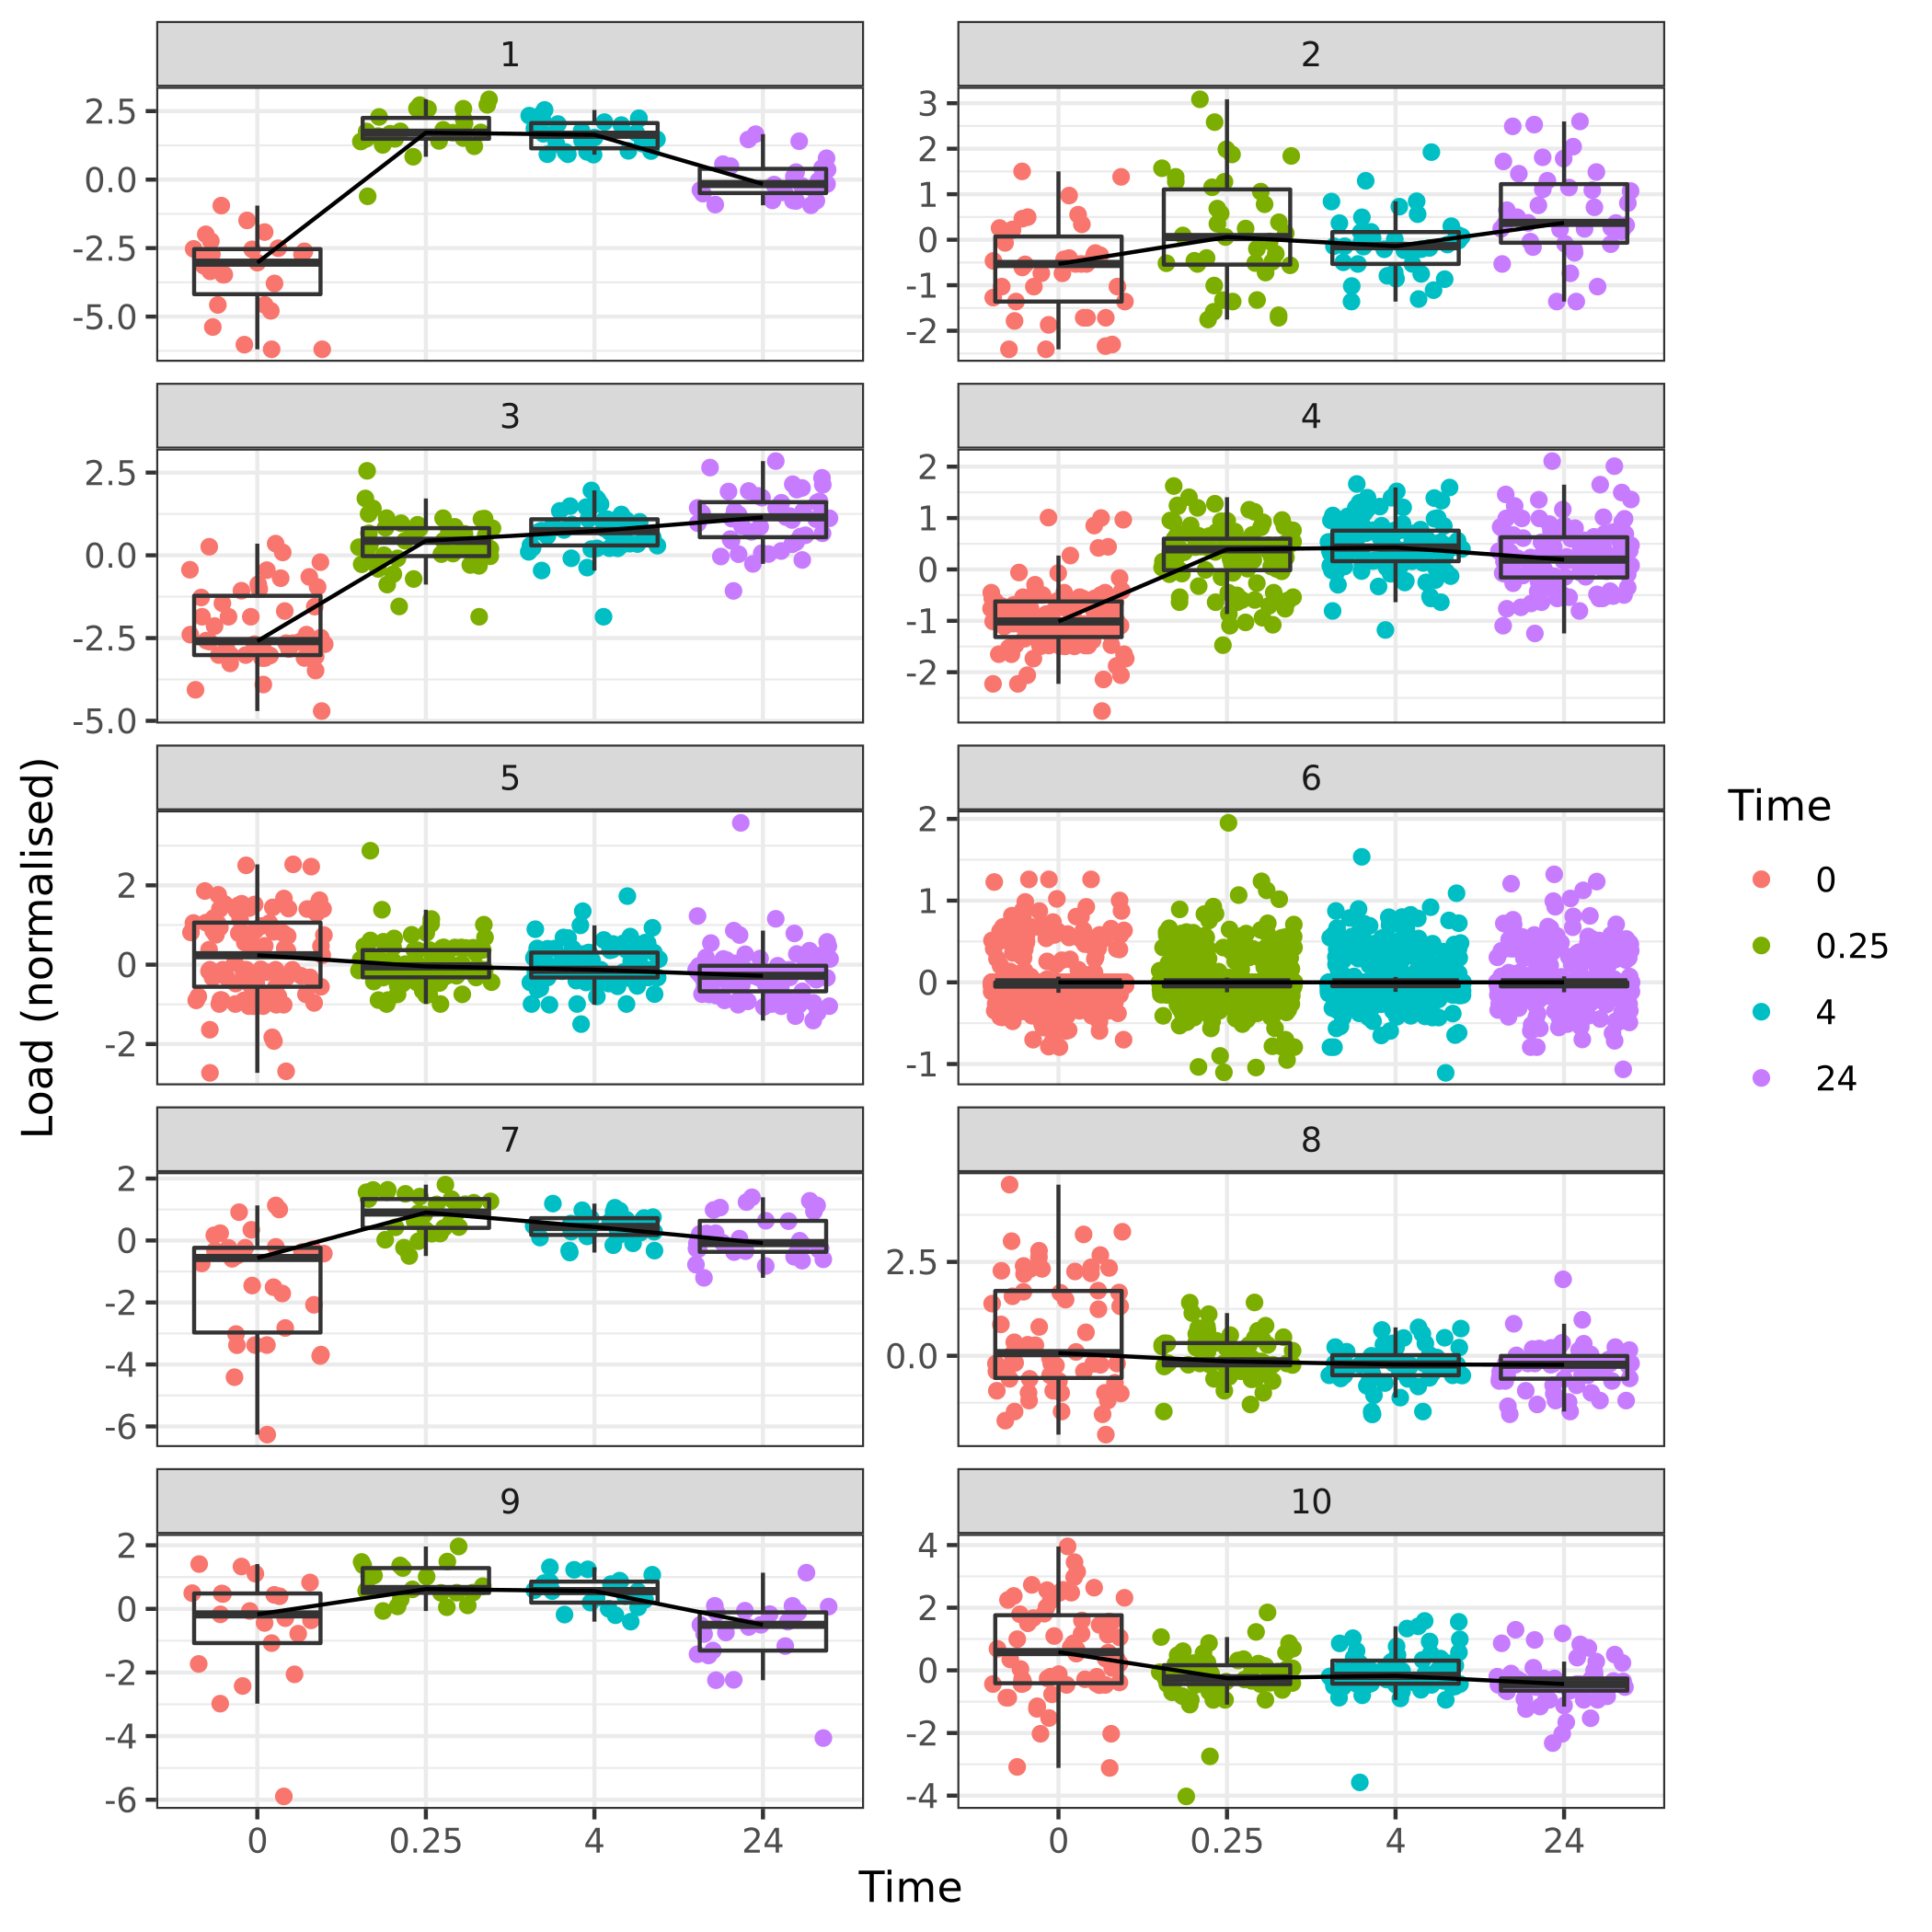
\includegraphics[width=.9\linewidth]{figure9/PERM/Legbox.png}
\end{center}
\begin{enumerate}
\item Supplemental Tables
\label{sec:orga3ff383}
\url{figure9/PERM/Legbox}
\end{enumerate}
\subsection{Figure 10: Time Course Body}
\label{sec:org4ec7d66}
\subsubsection{DEET}
\label{sec:org154e56e}
\begin{center}
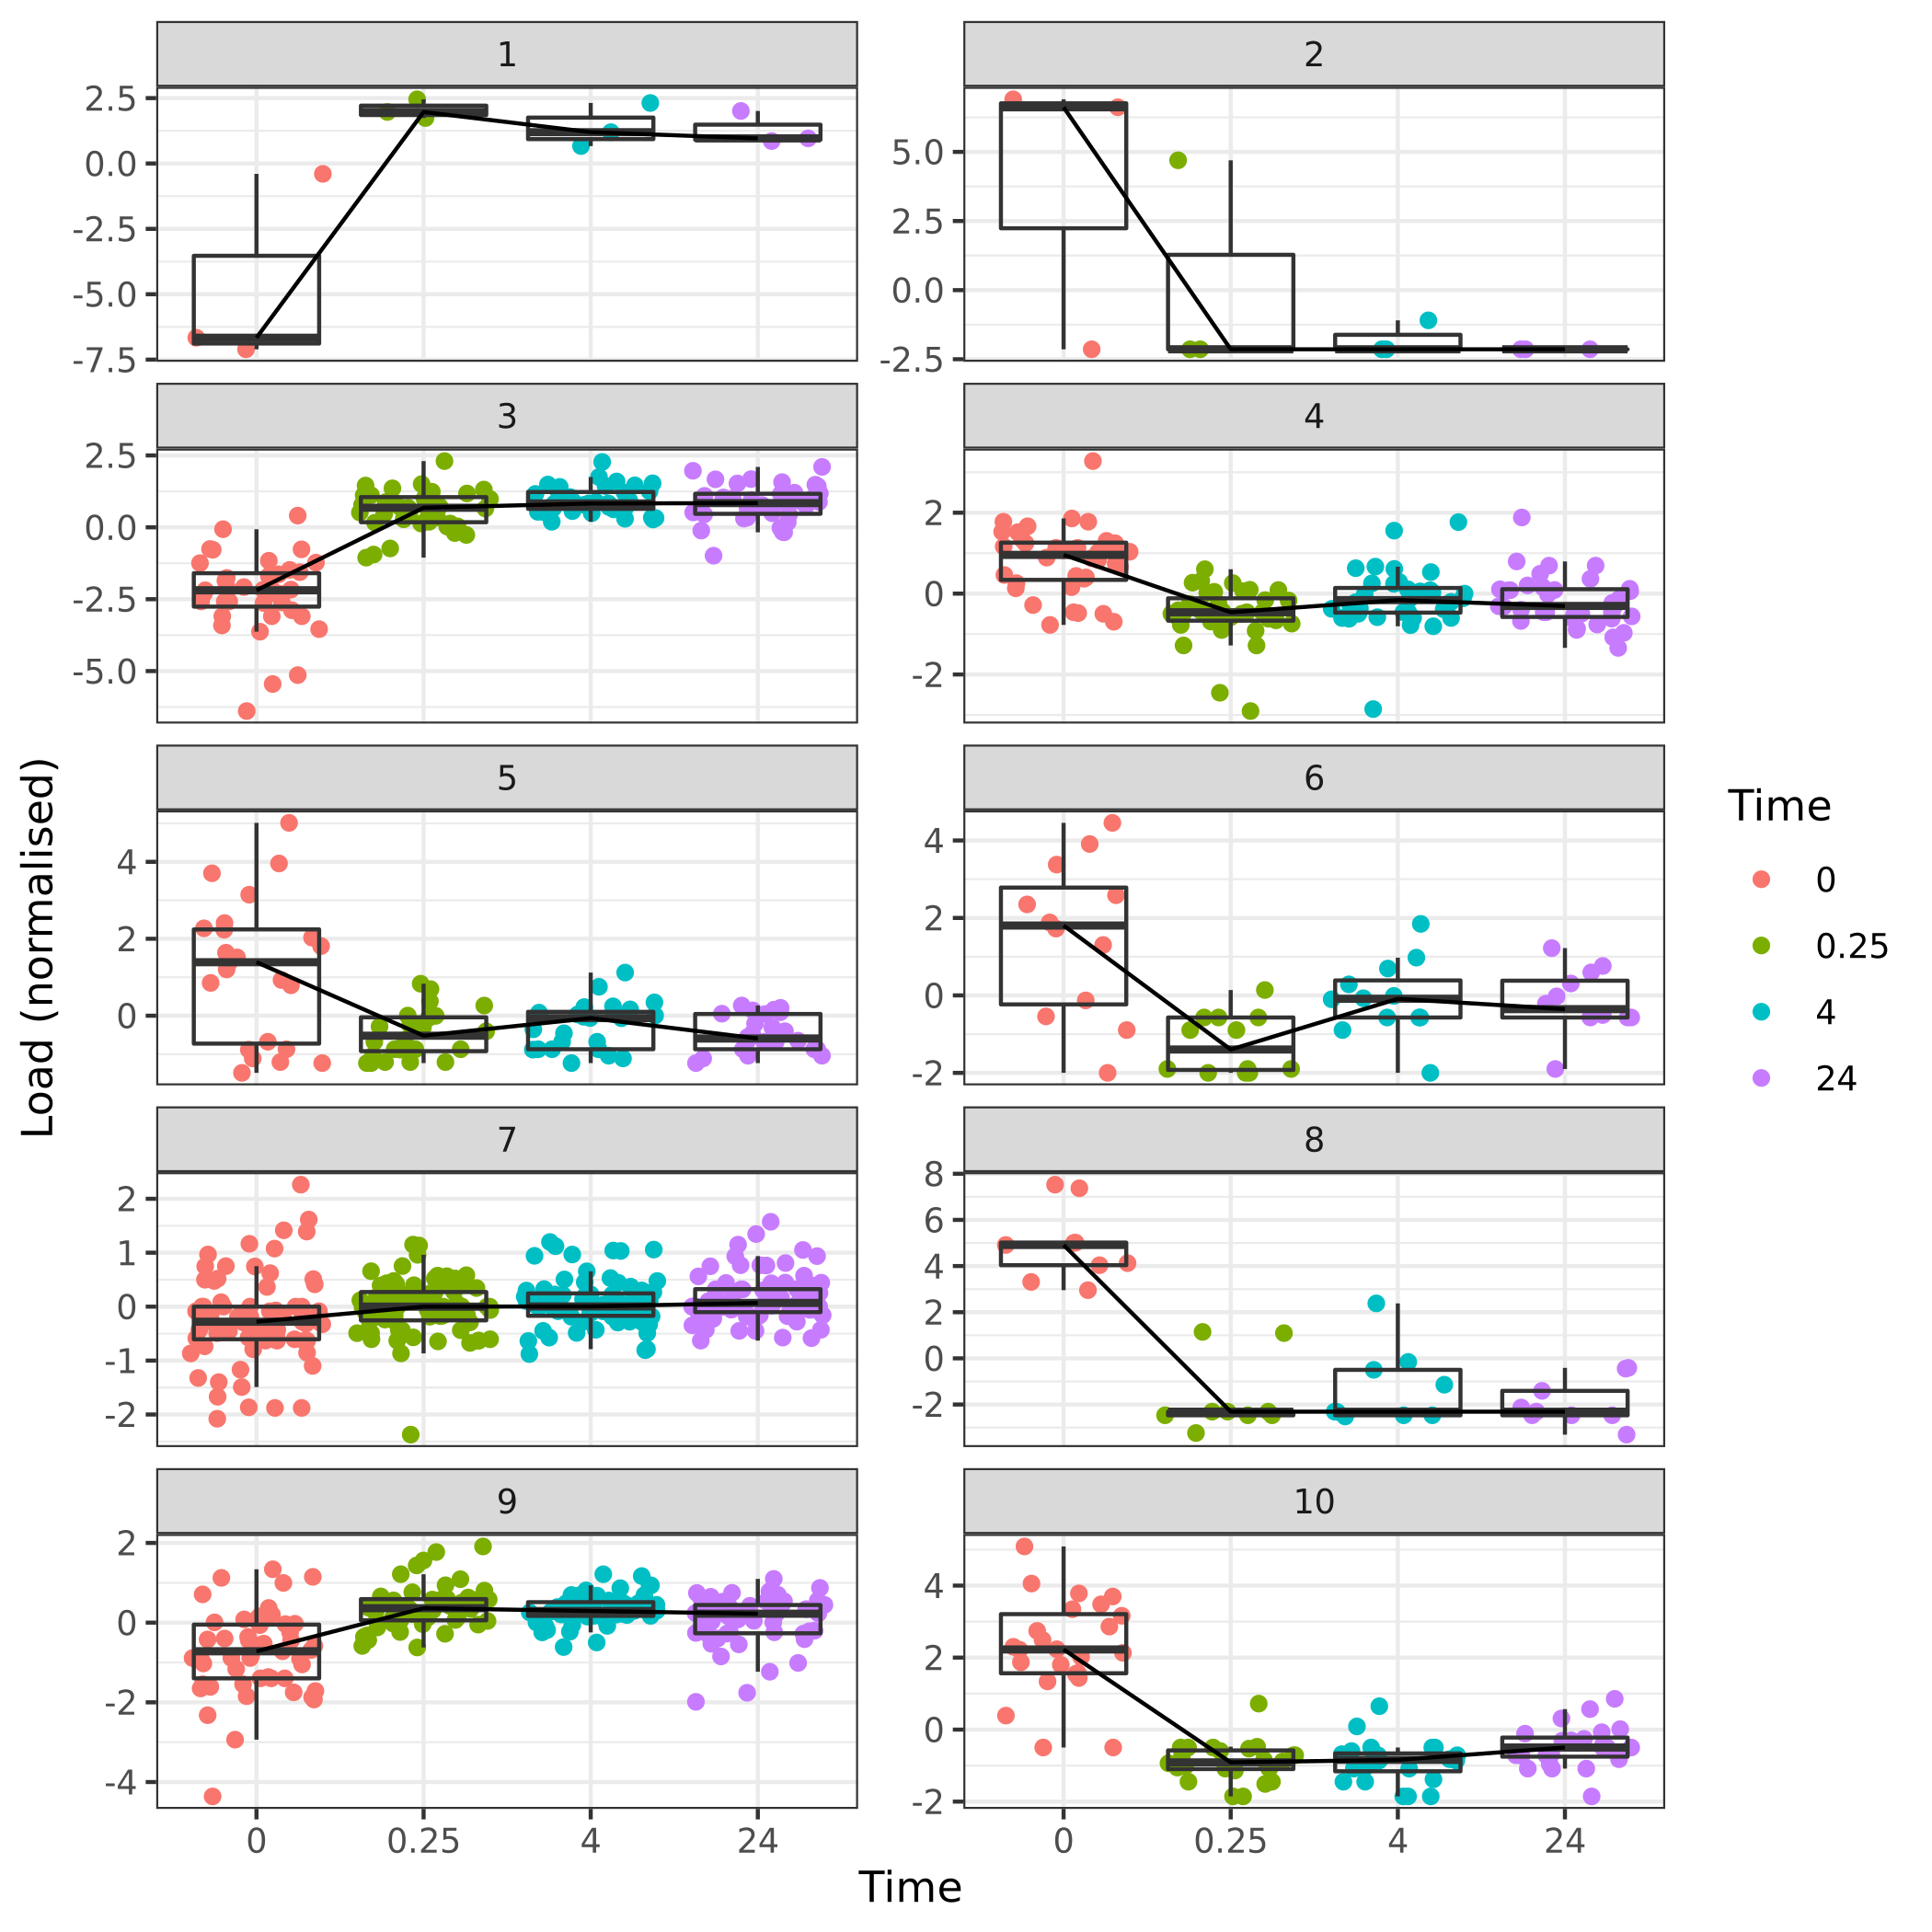
\includegraphics[width=.9\linewidth]{figure10/DEET/Bodybox.png}
\end{center}
\begin{enumerate}
\item Supplemental Tables
\label{sec:orge4a5927}
\url{figure10/DEET/Bodybox/}
\end{enumerate}
\subsubsection{PERM}
\label{sec:org006767e}
\begin{center}
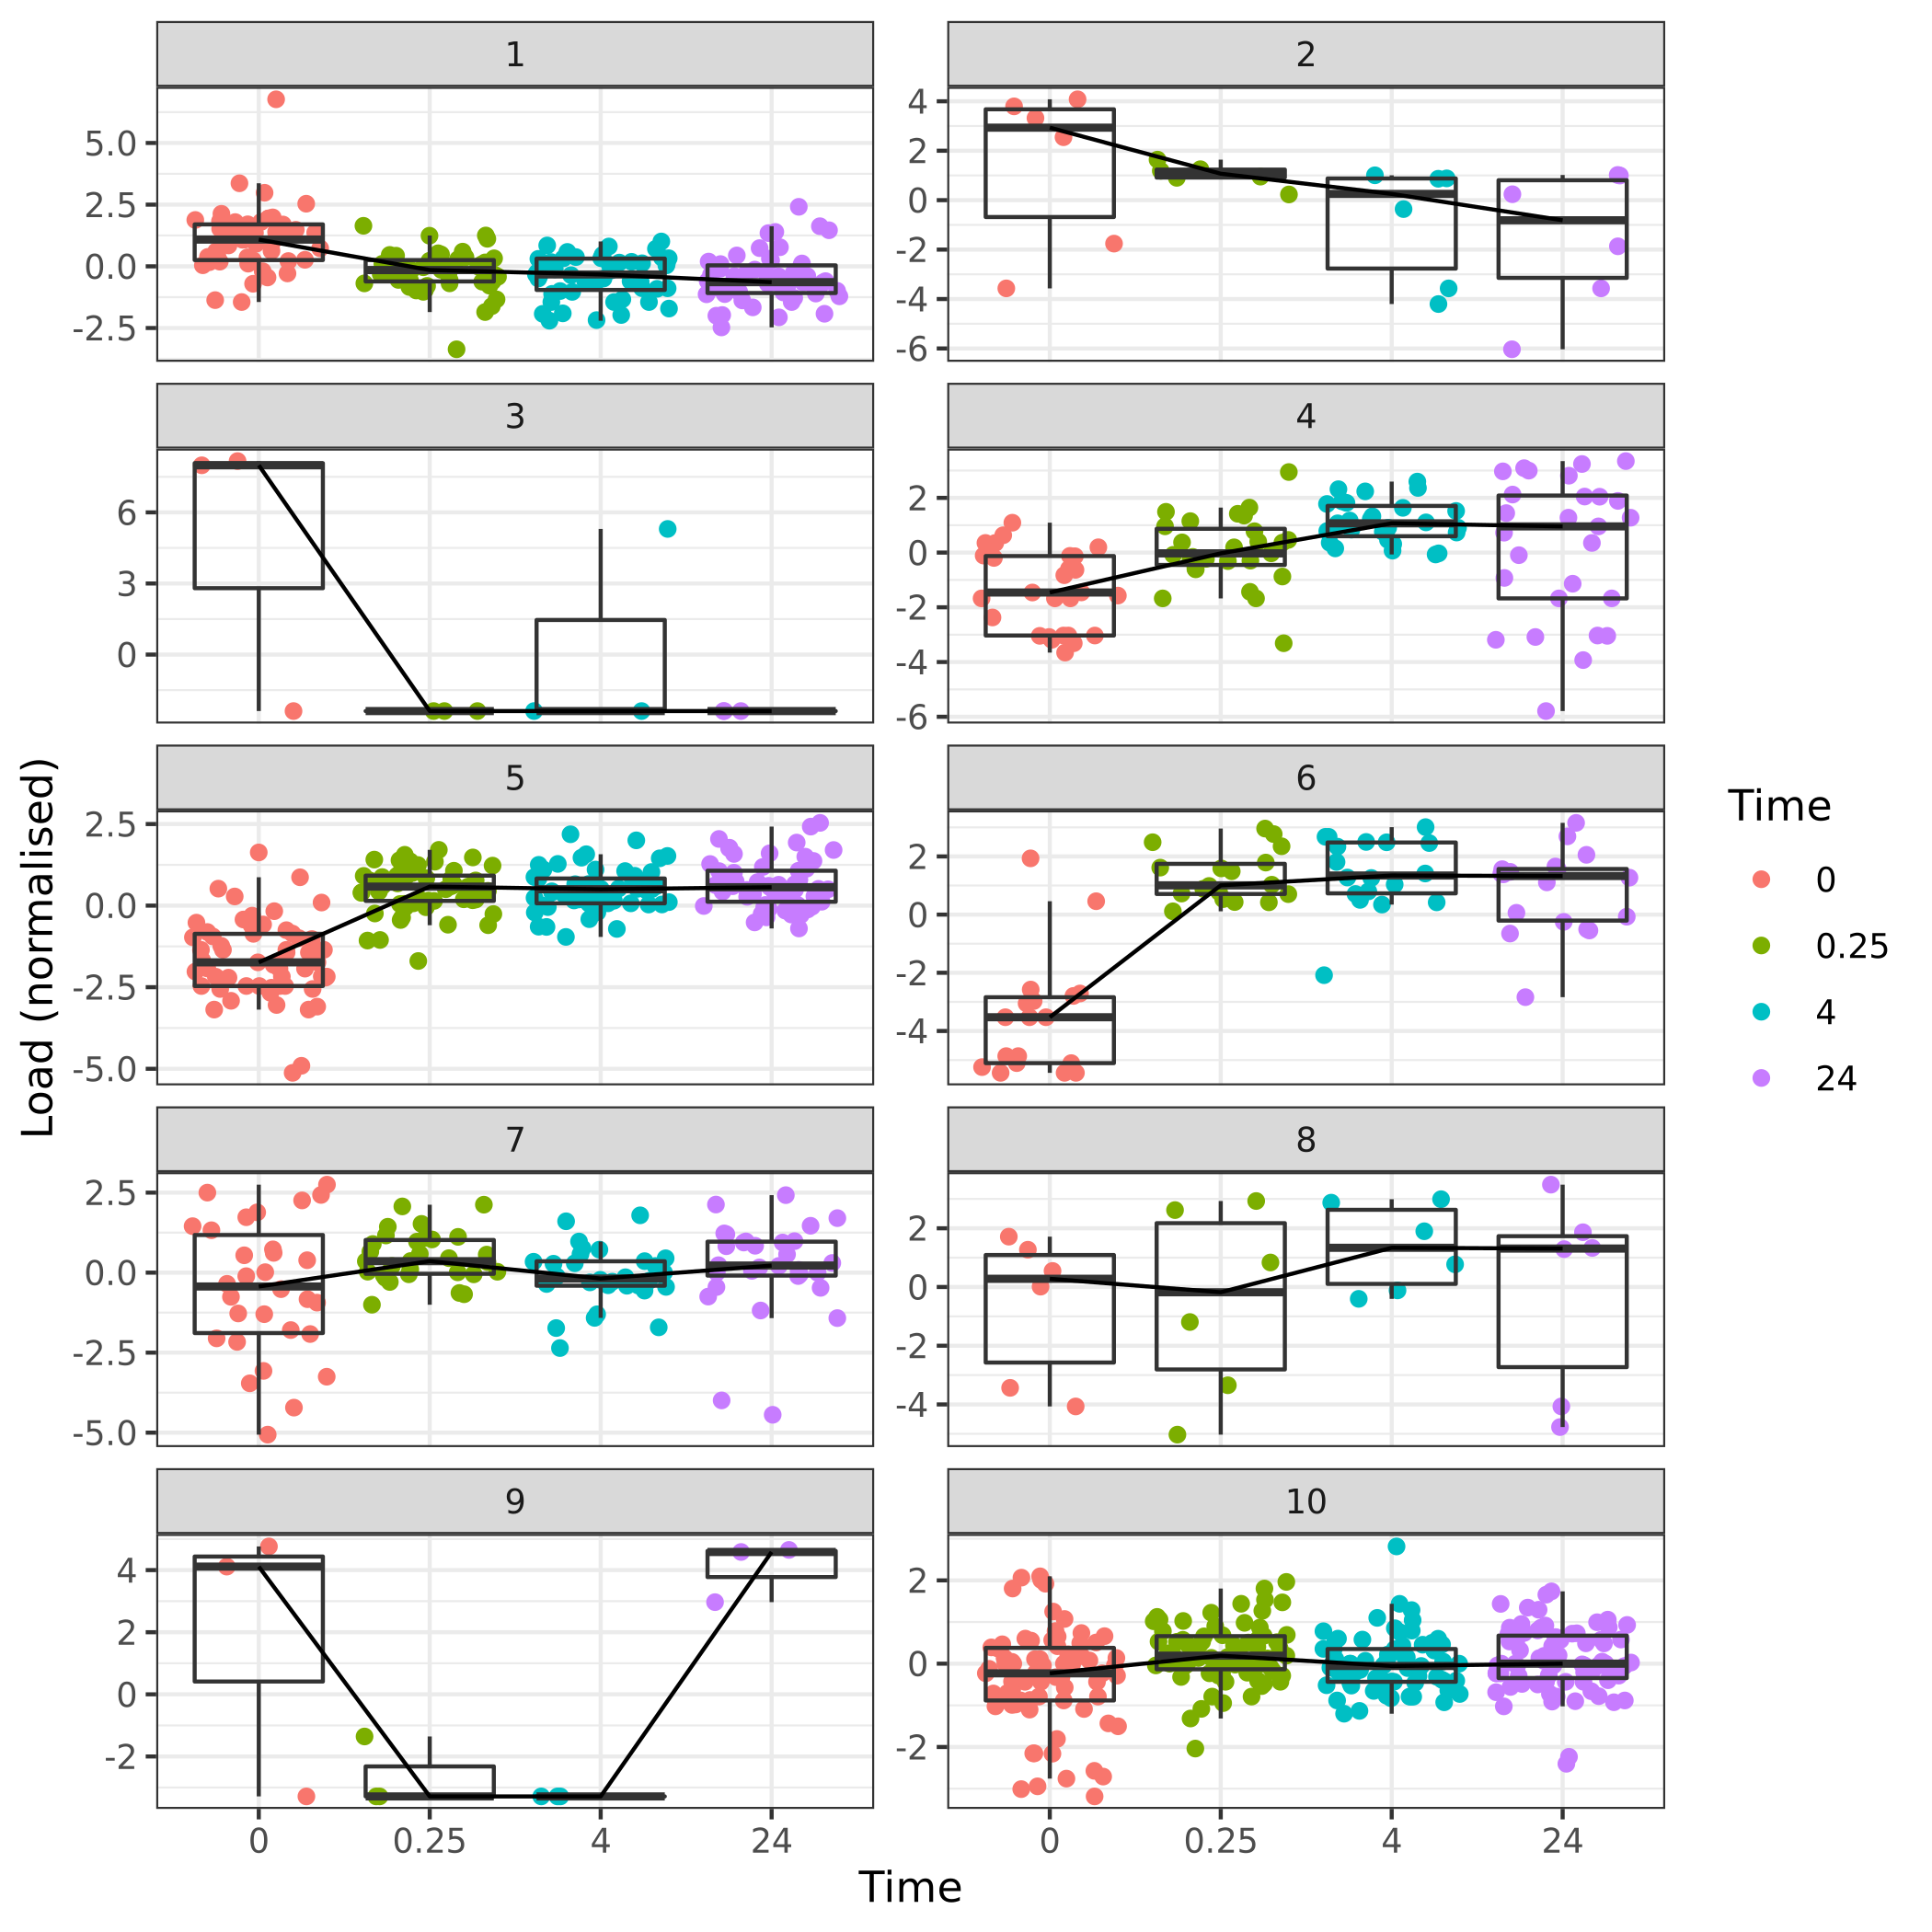
\includegraphics[width=.9\linewidth]{figure10/PERM/Bodybox.png}
\end{center}
\begin{enumerate}
\item Supplemental Tables
\label{sec:orgac21821}
\url{figure10/PERM/Bodybox/}
\end{enumerate}

\section{Discussion}
\label{sec:org9142f67}
\end{document}
